\documentclass[letterpaper,12pt]{scrartcl}
\usepackage{epsfig,latexsym,amsmath,amssymb,epic,eepic,psfrag,subfigure,float,euscript,array}
\usepackage[latin1]{inputenc}
\usepackage[margin=24mm]{geometry}
\usepackage{enumitem}
\usepackage{tikz,pgf,pgfplots}
\usepgfplotslibrary{fillbetween}
\usetikzlibrary{decorations, arrows, patterns}

\usepackage{adjustbox}
\usepackage[amssymb]{SIunits}

\usepackage{array}
\newcolumntype{L}{>{\[}l<{\]}} % math-mode version of "l" column type

\newenvironment{exercise}[1][Problem]{\begin{trivlist} \item[\hskip
    \labelsep {\stepcounter{exerctr}\bfseries #1
      \arabic{exerctr}}]}{\end{trivlist}\vspace{10mm}}

\newcounter{exerctr}
\newcounter{abcctr}[exerctr]

\newcommand{\abc}{\noindent\vspace{1mm}\\ {\bf
    \stepcounter{abcctr}(\alph{abcctr})\ }}
\newcommand{\bbm}{\begin{bmatrix}}
\newcommand{\ebm}{\end{bmatrix}}
\newcommand{\point}[1]{\hfill {\bf (#1p)}\\ \vspace{-5mm}}
\newcommand{\ctrb}{\EuScript{S}}
\newcommand{\Lap}{\mathcal{L}}
\newcommand{\obsv}{\EuScript{O}}
\newcommand{\realdel}{\text{Re}}
\newcommand{\imagdel}{\text{Im}}
\newcommand{\bC}{\mathbb{C}}
\newcommand{\bR}{\mathbb{R}}
\newcommand{\bmpv}{\begin{minipage}[t]}
\newcommand{\bmps}{\begin{minipage}[t]{45mm}}
\newcommand{\bmpm}{\begin{minipage}[t]{90mm}}
\newcommand{\bmpl}{\begin{minipage}[t]{\textwidth}}
\newcommand{\emp}{\end{minipage}}
\newcommand{\mexp}[1]{\ensuremath{\mathrm{e}^{#1}}}
\newcommand*{\laplaceinv}[1]{\ensuremath{\mathcal{L}^{-1} \left\{#1\right\}}}
\newcommand*{\ztrf}[1]{\ensuremath{\mathcal{Z} \left\{#1\right\}}}
\newcommand*{\shift}{\ensuremath{\operatorname{q}}}
\newcommand*{\diff}{\ensuremath{\operatorname{p}}}

\newcommand\tikzmark[2]{\tikz[overlay, remember picture, anchor=base] \node (#1) {#2};}
\newcommand\tikzmathmark[2]{\tikz[remember picture, inner sep=0pt, outer sep=0pt, baseline, anchor=base] \node (#1) {\ensuremath{#2}};}


\addtolength{\topmargin}{-8mm}
%\textheight 22.5cm
%\oddsidemargin 1.3cm
%\evensidemargin 1.3cm

\makeatletter
\newcommand*{\rom}[1]{\expandafter\@slowromancap\romannumeral #1@}
\makeatother

\newcommand*\circled[1]{\tikz[baseline=(char.base)]{
            \node[shape=circle,draw,inner sep=2pt] (char) {#1};}}


\title{Computerized Control Final exam (28\%)}
\author{Kjartan Halvorsen}
\date{}

\begin{document}

\maketitle


\begin{description}
\item[Time] Wednesday November 28 19:10 --- 21.55
\item[Place] 4206
\item[Permitted aids] The single colored page with your own notes, table of Laplace transforms, calculator
\end{description}

All answers should be readable and well motivated (if nothing else is written). Solutions/motivations should be written on the provided spaces in this exam. Use the last page if more space is needed.

\begin{center}
{\Large Good luck!} \\
\end{center}

\noindent
\fbox{
\bmpl%
{\bf Matricula and name:}\\
\vspace*{18mm}
\emp}


\clearpage

%-----------------------------------------------------------------
% Exercise 1. Block-diagram calculations
%-----------------------------------------------------------------
\begin{exercise}

The figure below shows a block-diagram of a two-degrees-of-freedom control system. 
\begin{center}
\includegraphics[width=0.6\linewidth]{../../homework/2dof-block-complete}
\end{center}

Which of the following pulse transfer operators describes the \textbf{closed-loop response}, $y(kh)$, to the measurement noise sequence $n(kh)$? No motivation required.
\begin{enumerate}
\item \( H_n(q) = \frac{1}{1 + H(q)F_b(q)} \)
\item \( H_n(q) = -\frac{H(q)F_f(q)}{1 + H(q)F_f(q)} \)
\item \( H_n(q) = -\frac{H(q)F_b(q)}{1 + H(q)F_b(q)} \)
\item \( H_n(q) = \frac{H(q)F_b(q)}{1 + H(q)F_b(q)} \)
\end{enumerate}

\end{exercise}

% -----------------------------------------------------------------
% Exercise 2. Match pulse-transfer function with step-response
%-----------------------------------------------------------------
\begin{exercise}

For each of the four pulse-transfer functions below, determine which of the step-responses in figure \ref{fig:steps} it corresponds to.
\begin{align*}
  G_1(z) &= \frac{0.026z + 0.024}{z(z-0.95)}\\
  G_2(z) &= \frac{0.13z + 0.12}{z^2 - z + 0.25}\\
  G_3(z) &= \frac{0.54z + 0.52}{{(z-0.5)}^2 + 0.81}\\
  G_4(z) &= \frac{0.025z + 0.025}{{(z-0.8)}^2 - 0.09}
\end{align*}

%\begin{center}
%\includegraphics[height=0.3\textheight]{../../figures/zgrid-crop}\\
%\end{center}

\begin{figure}[hbtp]
\begin{center}
\includegraphics[width=\linewidth]{step-responses}
\caption{Exercise \arabic{exerctr} Match the step-responses with the pulse-transfer functions.}\label{fig:steps}
\end{center}
\end{figure}

\noindent
\fbox{
\bmpl%
{\bf Motivation:}\\
\vspace*{120mm}
\emp}

\end{exercise}


% --------------------------------------------------------------------------------
% Match pulse-transfer function with difference equations
%--------------------------------------------------------------------------------

\begin{exercise}
A discrete-time LTI with input $u(k)$ and output $y(k)$ can be represented as a linear difference equation, or with a transfer operator $H(\shift)$, where $y(k) = H(\shift)u(k)$.  
In the table that follows, connect the pulse-transfer operator with the corresponding difference equation. No motivation required.

\def\tsep{5mm}
\begin{center}
\begin{tabular}{|p{5cm}p{8cm}|}
\hline
$H(\shift)$ & Difference equation\\\hline\hline
\vspace*{1mm}$\frac{b_0\shift+b_1}{\shift + a_1}$
& \vspace*{1mm}$y(k+1) = -a_1y(k) + b_0u(k) + b_1u(k-1)$\\[\tsep]
$\frac{b_0\shift+b_1}{\shift + a_1}\shift^{-1}$
& $y(k+1) = -a_1y(k-1) + b_0u(k-1) + b_1u(k-2)$\\[\tsep]
$\frac{b_0\shift+b_1}{\shift^2 + a_1}$
& $y(k+1) = -a_1y(k) + b_0u(k+1) + b_1u(k)$\\[\tsep]
$\frac{b_0\shift+b_1}{\shift^2 + a_1}\shift^{-1}$
& $y(k+1) = -a_1y(k-1) + b_0u(k) + b_1u(k-1)$\\[\tsep]\hline
\end{tabular}
\end{center}
\end{exercise}

\begin{exercise}
  A continuous-time lead-compensator 
  \begin{equation}
    F(s) = 10\frac{s+1}{s+4}
    \label{eq:lead}
  \end{equation}
  has been designed to control a plant $G(s)$. 
  \begin{center}
  \begin{tikzpicture}[scale = 0.8, node distance=22mm, block/.style={rectangle, draw, minimum width=15mm}, sumnode/.style={circle, draw, inner sep=2pt}]
    
    \node[coordinate] (input) {};
    \node[sumnode, right of=input, node distance=12mm] (sum) {\tiny $\sum$};
     \node[block, right of=sum, node distance=28mm] (controller) {$F(s)$};
     \node[block, right of=controller, node distance=38mm] (plant) {$G(s)$};
     \node[coordinate, right of=plant, node distance=35mm] (output) {};

     \draw[->] (input) -- node[above, pos=0.3] {$y_{ref}$} (sum);
     \draw[->] (sum) -- node[above, pos=0.3] {$$} (controller);
     \draw[->] (controller) -- node[above, pos=0.3] {$$} (plant);
     \draw[->] (plant) -- node[coordinate] (measure) {} node[above, very near end] {$y$} (output);
     \draw[->] (measure) -- ++(0, -2) -| node[pos=0.95, left] {$-$} (sum);

   \end{tikzpicture}
 \end{center}
 The continuous-time lead-compensator is discretized using the backward Euler approximation \[\frac{d}{dt} \approx \frac{\shift -1}{h\shift}.\]

\abc Which of the below pulse-transfer functions is the correct one (circle)? No motivation required.
 \begin{align*}
   F_d(z) &= 10\frac{z(1+h)-1}{z(1+4h)-1}\\[2mm]
   F_d(z) &= 10\frac{z(1+4h)-1}{z(1+h)-1}\\[2mm]
   F_d(z) &= 10\frac{z+1}{z+4}\\[2mm]
   F_d(z) &= 10\frac{z(1+h)-1}{z(1+h)-4}\\[2mm]
 \end{align*}

\pgfmathsetmacro\omegac{2}
\pgfmathsetmacro\hh{0.2}
\pgfmathsetmacro\argF{atan2(\omegac, 1) - atan2(\omegac, 4)}
\pgfmathsetmacro\argFd{atan2( (1+\hh)*sin(deg(2*\hh)), (1+\hh)*cos(deg(2*\hh))-1) 
 - atan2(  (1+4*\hh)*sin(deg(2*\hh)), (1+4*\hh)*cos(deg(2*\hh))-1 )} 

 \abc [Bonus problem worth 4p] The purpose of using a lead-compensator, as compared to a simpler proportional controller, is to improve the stability of the closed-loop system. The frequency response $F(i\omega)$ of the lead-compensator has positive phase, which improves the phase-margin of the system. Assuming that the cross-over frequency is $\omega_c = \unit{2}{\radian\per\second}$, the proposed lead-compensator \eqref{eq:lead} has a phase of 
\[ \arg F(i\omegac) = \arg 10 + \arg (i\omegac + 1) - \arg(i\omegac + 4) = \unit{\argF}{\degree}\]
at the cross-over frequency.
If the sampling period is $h=0.2$. What is the phase of the discretized filter $F_d(z)$ at the cross-over frequency? [You get 2p for answering correctly whether the phase of the discretized controller is larger or smaller than that of the continuous-time controller.]

\noindent
\fbox{
\bmpl%
{\bf Calculations and answer:}\\
\vspace*{70mm}
%\argFd
\emp}




\end{exercise}

%-------------------------------------------------------------------------------------------------
% State-space 
%-------------------------------------------------------------------------------------------------
\begin{exercise}
\abc%
Consider the first-order difference equation \(x(k+1) = ax(k) + bu(k)\). Which of the following is the correct expression for this discrete-time system in the z-domain? No motivation required.
\begin{align}
  X(z) &= (z-a)z^{-1}bU(z)\\
  X(z) &= z{(z-a)}^{-1}bU(z)\\
  X(z) &= {(z-a)}^{-1}bU(z)\\
  X(z) &= (z-a)bU(z)\\
\end{align}

\abc%
Consider the discrete-time DC-motor model
\pgfmathsetmacro\hh{0.2}
\pgfmathsetmacro\expminh{exp(-\hh)}
\pgfmathsetmacro\oneminexpminh{1-\expminh}
\pgfmathsetmacro\aoneone{\expminh}
\pgfmathsetmacro\atwoone{\oneminexpminh}
\pgfmathsetmacro\bone{\oneminexpminh}
\pgfmathsetmacro\btwo{\hh - 1+\expminh}
\begin{equation*}
  \begin{aligned}
    x(k) &= \bbm \pgfmathprintnumber[fixed,precision=1]{\aoneone} & 0\\
    \pgfmathprintnumber[fixed,precision=1]{\atwoone} & 1\ebm x(k)
    + \bbm \pgfmathprintnumber[fixed,precision=1]{\bone}\\
\pgfmathprintnumber[fixed,precision=2]{\btwo}\ebm u(k)\\
    y(k) &= \bbm 0 & 1 \ebm x(k),
  \end{aligned}
\end{equation*}
where \(x_1(k)\) is the angular velocity and \(x_2(k)\) is the angular position of the motor shaft.
Which of the below is the correct characteristic equation of the model? Motivate!
\begin{enumerate}
\item \((z-0.8)(z+1) = 0\)
\item \((z-0.8)(z-1) = 0\)
\item \((z+0.8)(z+1) = 0\)
\item \((z+0.8)(z-1) = 0\)
\end{enumerate}

\noindent
\fbox{
\bmpl%
{\bf Motivation:}\\
\vspace*{50mm}
\emp}

 
\abc%
If we attempt to control the DC-motor with the control law 
\begin{center}
\begin{adjustbox}{margin=1cm}
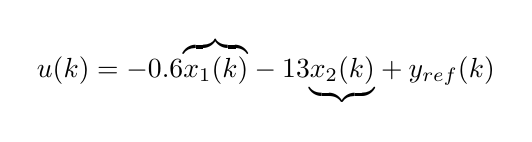
\begin{tikzpicture}
\node {$u(k) = -0.6\tikzmathmark{angvel}{\overbrace{x_1(k)}} - 13\tikzmathmark{angpos}{\underbrace{x_2(k)}} + y_{ref}(k)$};
\end{tikzpicture}
\end{adjustbox}
\end{center}
\tikz[overlay, remember picture] \draw[<-, thin] (angvel) -- ++(1cm,1cm) node[right] {angular velocity};
\tikz[overlay, remember picture] \draw[<-, thin] (angpos) -- ++(1cm,-1cm) node[right] {angle};

which poles will the closed-loop poles have? No motivation required.
\begin{enumerate}
\item \( z = 0.71 \pm 0.70 i\)
\item \( z_1 = 0.7, \; z_2 = 0.7\)
\item \( z_1 = 0, \; z_2 =  0\)
\item \( z_1 = 0, \; z_2 =  0.7\)
\end{enumerate}

\abc%
Discuss in 2-3 sentences the properties of the closed-loop system obtained in \textbf{(c)}. 

\noindent
\fbox{
\bmpl%
{\bf Properties of the closed-loop system:}\\
\vspace*{50mm}
\emp}


\end{exercise}

%\cleardoublepage 
%\end{document}


\section*{Solutions}

\setcounter{exerctr}{0} 

\begin{exercise}
Using Mason's rule, which says that the numerator of the closed-loop pulse-transfer function equals the gain in the direct path from the input signal to the output signal, it is clear that the answer must be \( H_n(q) = -\frac{H(q)F_b(q)}{1 + H(q)F_b(q)} \).
\end{exercise}


\begin{exercise}
\pgfmathsetmacro{\omegan}{sqrt(1+pow(0.6, 2))}
\pgfmathsetmacro{\omeganhertz}{\omegan * 1000/2/pi}
\pgfmathsetmacro{\hh}{0.2}
\pgfmathsetmacro{\pdreal}{exp(-\hh)*cos(deg(0.6*\hh))}
\pgfmathsetmacro{\pdim}{exp(-\hh)*sin(deg(0.6*\hh))}

The idea is to figure out the poles of the four systems, and from this determine how the system should respond.

The system $G_1(z)$ poles in $z=0$ and $z=0.95$, the latter of which is dominating. This gives a slow first-order response. The system $G_2(z)$ is critically damped with two poles in $z=0.5$. This has a stable, fast response with no overshoot. System $G_3(z)$ has two poles in $z = 0.5 \pm i0.9$ which are outside the unit circle. This gives an oscillating, unstable response. Finally, $G_4(z)$ has poles in $z=0.5$ and $z=1.1$. This gives an unstable response without oscillations. The analysis leads to the pairing: \textbf{$G_1(z)$ --- \rom{1}},  \textbf{$G_2(z)$ --- \rom{3}},  \textbf{$G_3(z)$ --- \rom{4}},  \textbf{$G_4(z)$ --- \rom{2}}. 
\end{exercise}

\begin{exercise}
The z-transform can be used in this exercise to find the correct answer, or more directly to just write the difference equation using the shift operator. For instance, the first difference equation becomes
\[ y(k+1) = -a_1y(k) + b_0u(k) + b_1u(k-1)\]
\[ (\shift + a_1)y(k) = (b_0 + b_1\shift^{-1}) u(k)\]
\[ y(k) = \frac{b_0\shift + b_1}{\shift + a_1}\shift^{-1} u(k).\]
The complete answer is
%\end{exercise}
%\end{document}
\def\tsep{5mm}
\begin{center}
\begin{tabular}{|p{5cm}p{8cm}|}
\hline
$H(\shift)$ & Difference equation\\\hline\hline
\vspace*{1mm}$\frac{b_0\shift+b_1}{\shift + a_1}$\tikzmark{H1}{}
& \vspace*{1mm}\tikzmark{sys1}{}{$y(k+1) = -a_1y(k) + b_0u(k) + b_1u(k-1)$}\\[\tsep]
$\frac{b_0\shift+b_1}{\shift + a_1}\shift^{-1}$\tikzmark{H2}{}
& \tikzmark{sys2}{}{$y(k+1) = -a_1y(k-1) + b_0u(k-1) + b_1u(k-2)$}\\[\tsep]
$\frac{b_0\shift+b_1}{\shift^2 + a_1}$\tikzmark{H3}{}
& \tikzmark{sys3}{}{$y(k+1) = -a_1y(k) + b_0u(k+1) + b_1u(k)$}\\[\tsep]
$\frac{b_0\shift+b_1}{\shift^2 + a_1}\shift^{-1}$\tikzmark{H4}{}
& \tikzmark{sys4}{}{$y(k+1) = -a_1y(k-1) + b_0u(k) + b_1u(k-1)$}\\[\tsep]\hline
\end{tabular}
\end{center}

\tikz[remember picture, overlay] \draw[<->, blue!60!black] (H1) to[out=0, in=180] (sys3); 
\tikz[remember picture, overlay] \draw[<->, orange!60!black] (H2) to[out=0, in=180] (sys1); 
\tikz[remember picture, overlay] \draw[<->, red!60!black] (H3) to[out=0, in=180] (sys4); 
\tikz[remember picture, overlay] \draw[<->, green!60!black] (H4) to[out=0, in=180] (sys2); 

\end{exercise}

\begin{exercise}
\abc%
To find the discretized controller using the backward Euler approximation, substitute $s = \frac{z-1}{zh}$ in the transfer function. This gives
\begin{equation*}
\begin{aligned}
  F_d(z) &= F(s)|_{s=\frac{z-1}{zh}} = 10 \frac{\frac{z-1}{zh} + 1}{\frac{z-1}{zh} + 4}\\
         &= 10 \frac{z-1 + zh}{z-1 + 4zh} = 10\frac{z(1+h) - 1}{z(1+4h) - 1}.
\end{aligned}
\end{equation*}

\abc%
In discrete-time, the frequency response of a pulse-transfer function is obtained by evaluating the pulse-transfer function on the upper half of the unit circle, i.e.~\(F_d(z=\mathrm{e}^{i\omega h}\), where $\omega$ is the continuous-time frequency and $h$ is the sampling period. The Bode-plot of a discrete-time system ends at the frequency corresponding to $z=\mathrm{e}^\pi$, which is the Nyquist frequency $\omega_N = \frac{\pi}{h}$. 

We are asked to determine the phase (argument) of the discrete-time pulse-transfer function at the frequency $\omega_c = \unit{2}{\radian\per\second}$, which means to determine $\arg F_d(\mathrm{e}^{i\omega_c h})$, which is
\pgfmathsetmacro\omegac{2}
\pgfmathsetmacro\hh{0.2}
\pgfmathsetmacro\argF{atan2(\omegac, 1) - atan2(\omegac, 4)}
\pgfmathsetmacro\argFd{atan2( (1+\hh)*sin(deg(2*\hh)), (1+\hh)*cos(deg(2*\hh))-1) 
 - atan2(  (1+4*\hh)*sin(deg(2*\hh)), (1+4*\hh)*cos(deg(2*\hh))-1 )} 
\begin{equation*}
  \begin{aligned}
    \arg F_d(\mathrm{e}^{i\omega_c h}) &= \arg 10 \frac{\mathrm{e}^{i\omega_c h}(1+h) - 1}{\mathrm{e}^{i\omega_c h}(1+4h) - 1}\\
 &= \arg 10 + \arg \big(\mathrm{e}^{i\omega_c h}(1+h) - 1\big) - \arg \big(\mathrm{e}^{i\omega_c h}(1+4h) - 1\big)\\
      &= 0 + \arg \big(\mathrm{e}^{i0.4}1.2 - 1\big) - \arg \big(\mathrm{e}^{i0.4}1.8 - 1\big)\\
       &= \arg\big( (1.2\cos(0.4)-1) + i1.2\sin(0.4) \big) - \arg\big( (1.8\cos(0.4)-1) + i1.8\sin(0.4)\big)\\
      &= \tan^{-1}\left(\frac{1.2\sin(0.4)}{1.2\cos(0.4)-1}\right) - \tan^{-1}\left(\frac{1.8\sin(0.4)}{1.8\cos(0.4)-1}\right) = \unit{\argFd}{\degree} < \unit{\argF}{\degree}.
  \end{aligned}
\end{equation*} 
\end{exercise}

\begin{exercise}
  \abc%
  Applying the z-transform to the difference equation $x(k+1) = ax(k) + bu(k)$ (assuming $x(0)=0$) gives
  \[ zX(z) = aX(z) + bU(z)\]
  \[ zX(z) - aX(s) = bU(z)\]
  \[ (z-a)X(z) = bU(z)\]
  \[ X(z) = {(z-a)}^{-1}bU(z) = \frac{b}{z-a}U(z).\]
  \abc%
  The poles of the system are the eigenvalues of the state-transition matrix 
  \[ \Phi = \bbm 0.8 & 0\\0.2 & 1\ebm.\]
  The eigenvalues are easy to determine here, since the matrix is triangular. They are found on the diagonal as $z=0.8$ and $z=1$. This means that the characteristic equation must be 
  \[ (z-0.8)(z-1) = 0. \]
  \abc%
  The suggested control-law is $u(k) = -0.6x_1(k) - 13x_2(k) + y_{ref}(k)$. Note the large gain in the feedback for the second state element, which is the angular position. The feedback gain for the first element, which is the angular velocity is much smaller. We should therefore expect a system with small damping. Only Case 1 fits: $z=0.71 \pm 0.70i$. You can of course also just calculate what the poles are from the characteristic equation for the closed-loop system $\det \left( zI - (\Phi - \Gamma L)\right) = 0$:
  \begin{equation*}
    \begin{aligned}
      \det\left( zI - (\Phi - \Gamma L) \right) &=  
          \det\left( \bbm z & 0\\ 0 & z\ebm  - \Big( \bbm 0.8 & 0\\0.2 & 1 \ebm - \bbm 0.2\cdot 0.6 & 0.2\cdot 13\\ 0.02\cdot 0.6 & 0.02\cdot 13\ebm\Big)\right)\\
          &= \det \bbm z-0.8+0.12 & 2.6\\-0.2 + 0.012 & z-1+0.26 \ebm\\
          &= (z-0.68)(z-0.74) + 2.6\cdot{}0.188) = z^2 -1.42z + 0.992\\
          &= (z-0.71-i0.70)(z-0.71+i0.70).
    \end{aligned}
  \end{equation*}
\abc%
The poles have magnitude \(|0.71+0.70i| = 0.997\), so the system is almost undamped. Any excitation of the system will give oscillations that die out very slowly. The frequency of the oscillations are given by 
\pgfmathsetmacro\argP{rad(atan2(0.70, 0.71))}
\pgfmathsetmacro\omegar{\argP/0.2}
\[ \omega_r h = \arg (0.71+0.70i) = \argP\]
which gives 
\[ \omega_r = \unit{\omegar}{\radian\per\second}.\]
\end{exercise}
\end{document}
